\section{Datenpipeline}

Im nachfolgenden Teil der Arbeit werden die einzelnen Elemente der erstellte Datenpipeline nun genauer besprochen und erläutert. Dazu wird in Abbildung \ref{fig:datenpipelineFull} zunächst die Datenpipeline als Ganzen betrachtet.

\begin{figure}[h!]
    \vspace{1cm}
    \centering
    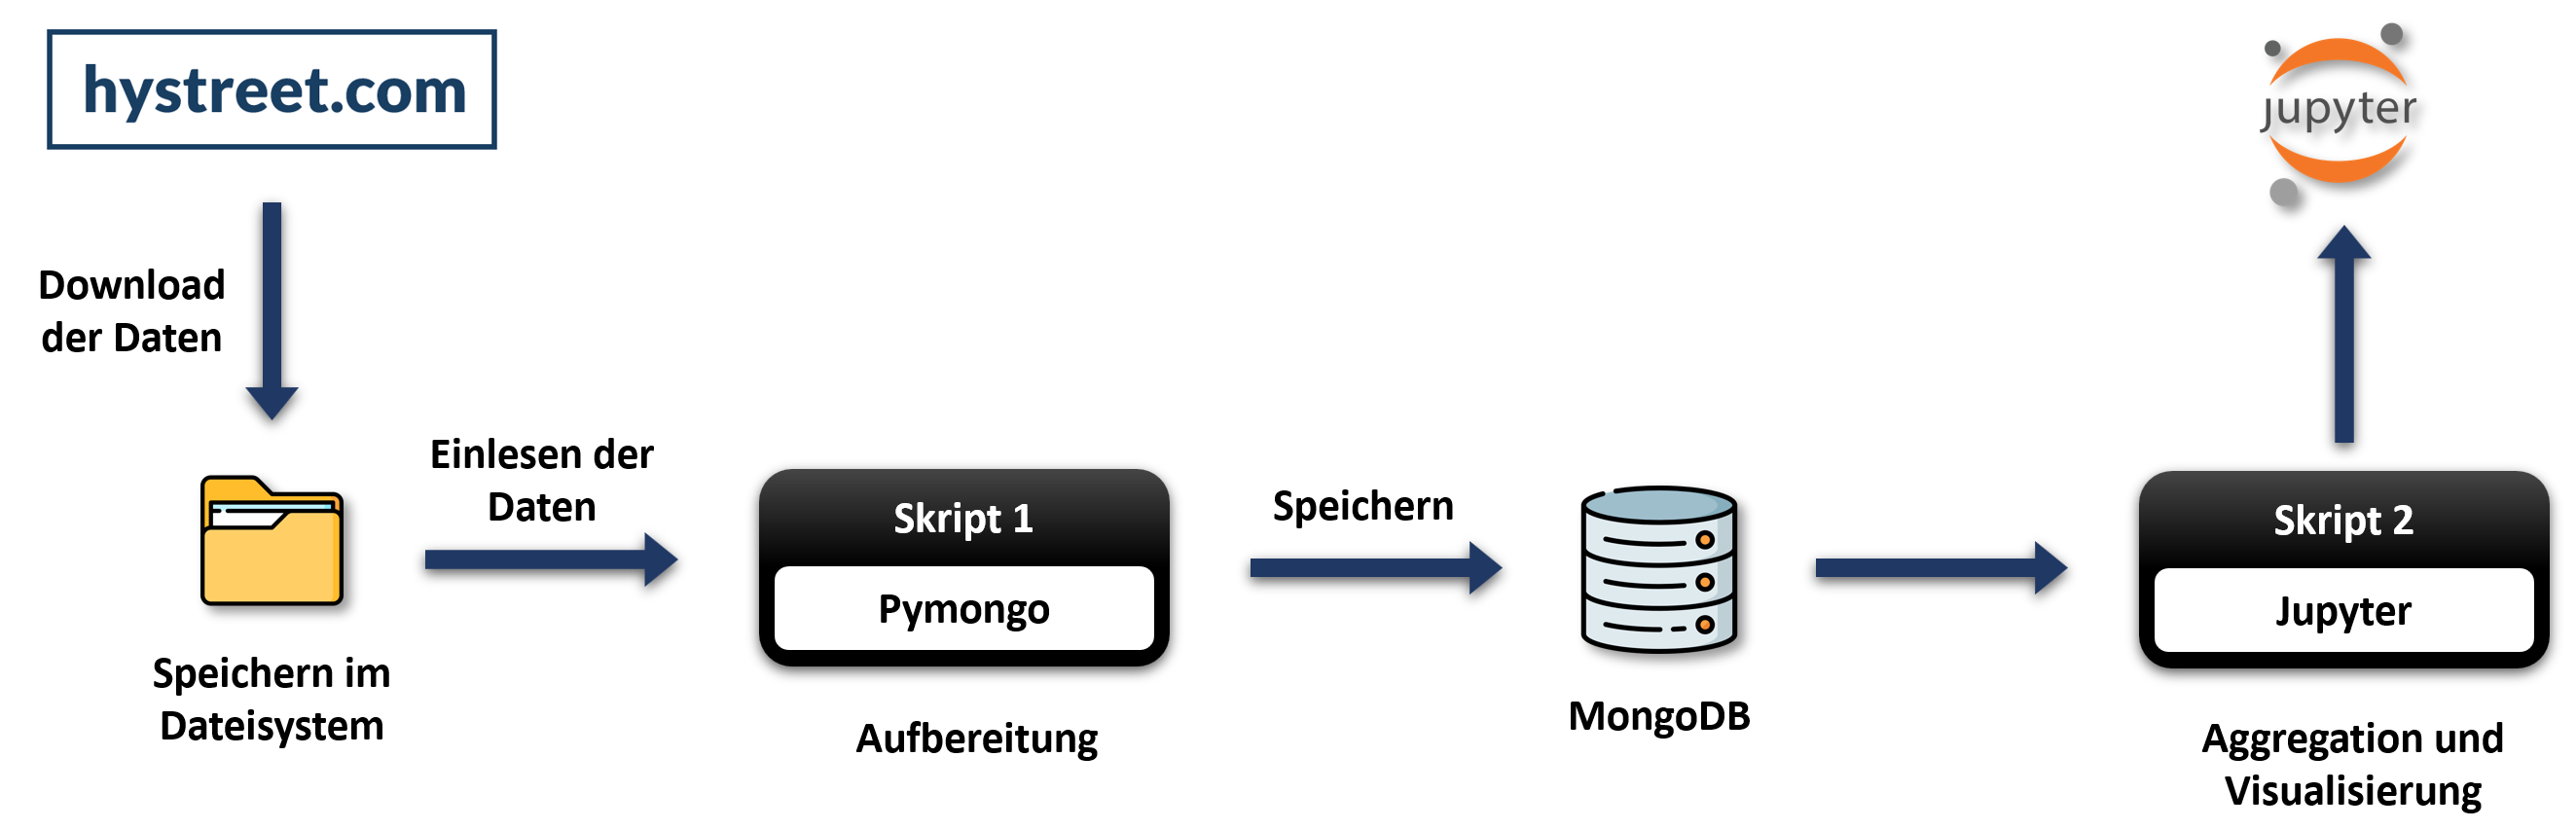
\includegraphics[width=0.9\linewidth]{images/datenpipeline.png}
    \caption{Datenpipeline zur Verarbeitung der HyStreet-Daten}
    \label{fig:datenpipelineFull}
    \vspace{0.5cm}
\end{figure}


Wie bereits erwähnt, stammen die Daten aus der Internetseite \href{https://hystreet.com}{HyStreet.com}. Die Webseite stellt somit auch den Startpunkt der Datenpipeline dar. Da die Daten nur kostenpflichtig automatisiert über eine API Schnittstelle heruntergeladen werden konnten, mussten wir uns für die Alternative entscheiden, die Daten manuell über deren Webseite herunterzuladen. Über den manuellen Download ist der Erhalt der Daten kostenlos. 
Zum genauen Vorgang des Downloads im folgenden Abschnitt Genaueres. Das Ergebnis dieses Schrittes ist eine Dateien im CSV-Format für den jeweiligen Standort. Der Aufbau dieser Dateien wurde bereits im einführenden Kapitel genauer beschrieben. Nach dem Herunterladen, werden die Dateien nun zunächst im lokalen Dateisystem gespeichert, um anschließend im Python Skript \emph{Skript 1} verarbeitet werden zu können.

In diesem Skript werden die Daten aus allen heruntergeladenen Dateien mit Hilfe des Packages \emph{Pandas} eingelesen und verarbeitet. Dabei werden diverse Spalten in ihre Einzelteile zerlegt und Spalten, die für unsere Zwecke nicht weiter erforderlich sind entfernt. Nach der Aufbereitung der Daten, werden diese schließlich in das JSON-Format umgewandelt, um im letzten Schritt in eine MongoDB eingelesen zu werden.


\subsection{Einlesen der Daten}